% ── Section 4.9 — null model: swapping the crisis assets ─────────────────────
\subsection{Null model: swapping the crisis assets}
\label{sec:null_swap}

A high $R^2$ between the empirical exposure $E_i$ and the SIS prediction $x_i$
is not, by itself, evidence that the model captures anything specific to asset
$i$: during a crisis rise both curves are increasing by construction, so
\emph{any} rising trajectory can trivially match any other. To measure how much
of the fit is genuinely asset-specific, we re-pair each empirical curve $E_i$
with the SIS trajectory $x_j$ of \emph{another} crisis asset, drawn by
derangement (a permutation with no fixed point, within groups of curves of
equal length; the two non-swappable singletons are excluded on both sides).
Repeating the draw $2\,000$ times yields the null distribution of the number of
curves with $R^2 > 0.6$, to be compared with the real pairing ($773$ swappable
curves over the $17$ crisis rises).

Figure~\ref{fig:null_swap} shows the result for the four methods
(Table~\ref{tab:null_swap} for the detailed counts). The real pairing beats the
null in every case, between $2.3\sigma$ and $4.1\sigma$ above it depending on
the method, the largest margin being for VAR(13) --- so the SIS prediction does
carry asset-specific information. The excess is however modest: swapping the
assets still leaves ${\sim}85\%$ of the well-fitted curves, which confirms that
the bulk of the $R^2$ comes from the common saturating shape of the crisis
rises, and only a thin margin from the identity of the asset itself. Any claim
based on the per-asset $R^2$ must therefore be read with this ceiling in mind.

\begin{figure}[t]
  \centering
  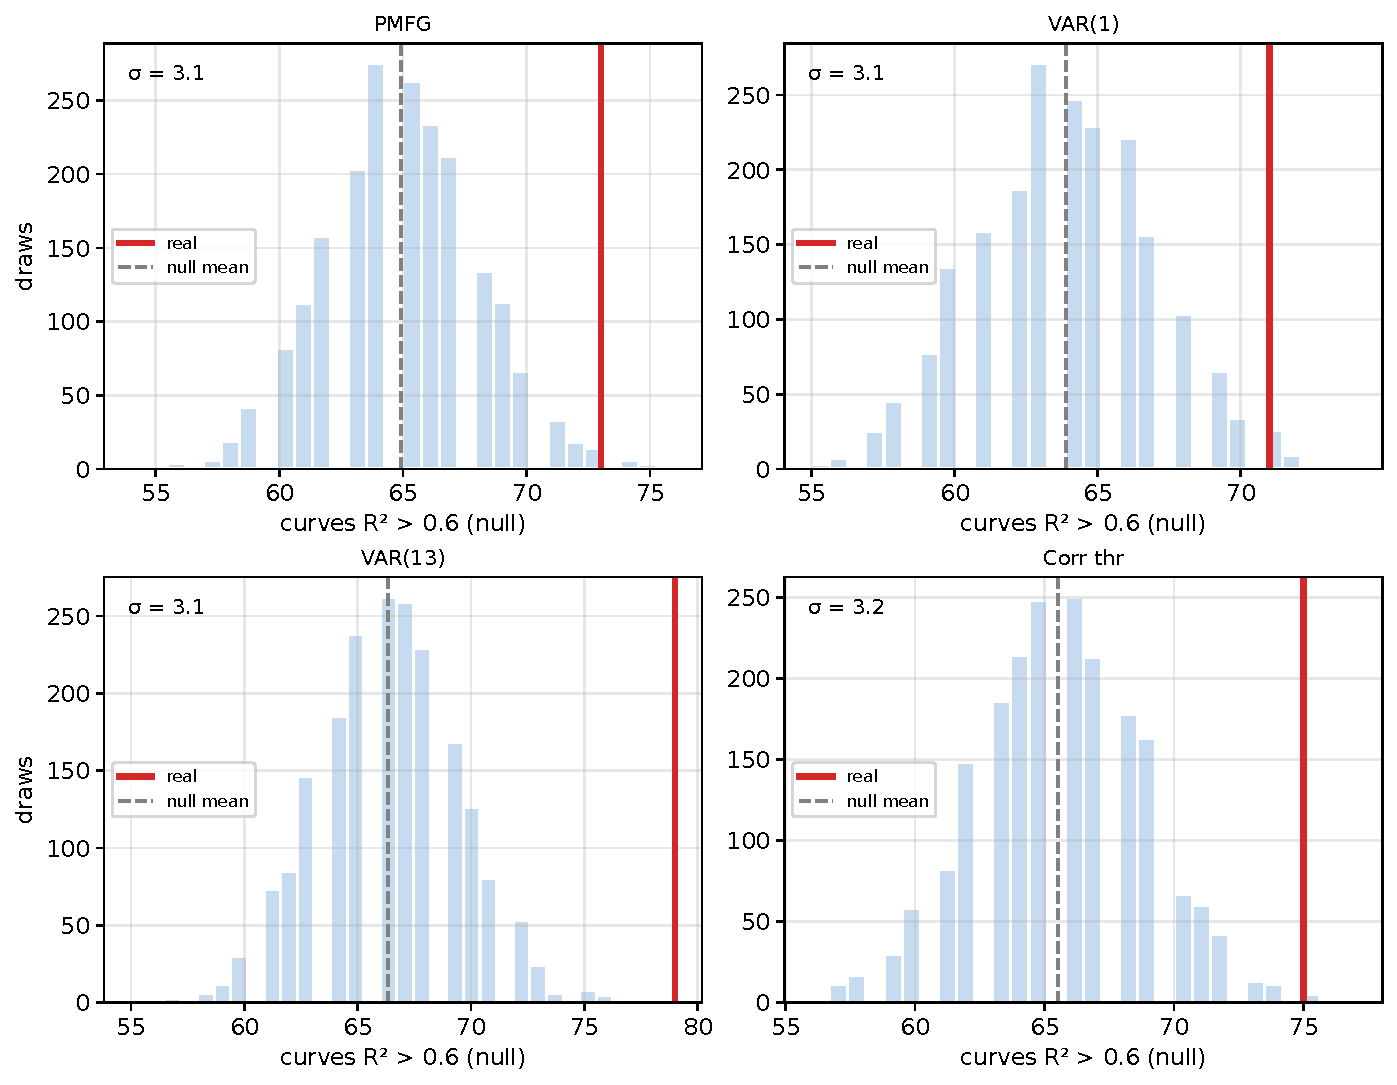
\includegraphics[width=0.85\textwidth]{Fig/rapport/fig_4_12_null_swap.pdf}
  \caption{Crisis-asset swap null: each empirical curve $E_i$ is re-paired with
  the SIS trajectory of another crisis asset (derangement within equal-length
  groups, $2\,000$ draws). Histograms: null distribution of the number of
  curves with $R^2 > 0.6$; red line: real pairing; dashed grey line: null mean.
  The real pairing is significantly above the null for all four methods
  ($2.3\sigma$--$4.1\sigma$), with the largest margin for VAR(13).}
  \label{fig:null_swap}
\end{figure}

\begin{table}[t]
  \centering
  \begin{tabular}{lrlr}
\toprule
method & real & null (mean ± sd) & z \\
\midrule
PMFG & 73 & 64.9 ± 3.1 & 2.61 \\
VAR(1) & 71 & 63.9 ± 3.1 & 2.29 \\
VAR(13) & 79 & 66.3 ± 3.1 & 4.11 \\
Corr thr & 75 & 65.6 ± 3.2 & 2.92 \\
\bottomrule
\end{tabular}

  \caption{Crisis-asset swap null, per method: real count of curves with
  $R^2 > 0.6$ ($773$ swappable curves), mean $\pm$ standard deviation of the
  null ($2\,000$ derangement draws), and deviation $z$ of the real count in
  units of the null standard deviation.}
  \label{tab:null_swap}
\end{table}
